\section{Dataset}
\label{dataset}
\begin{figure*}[!h]
  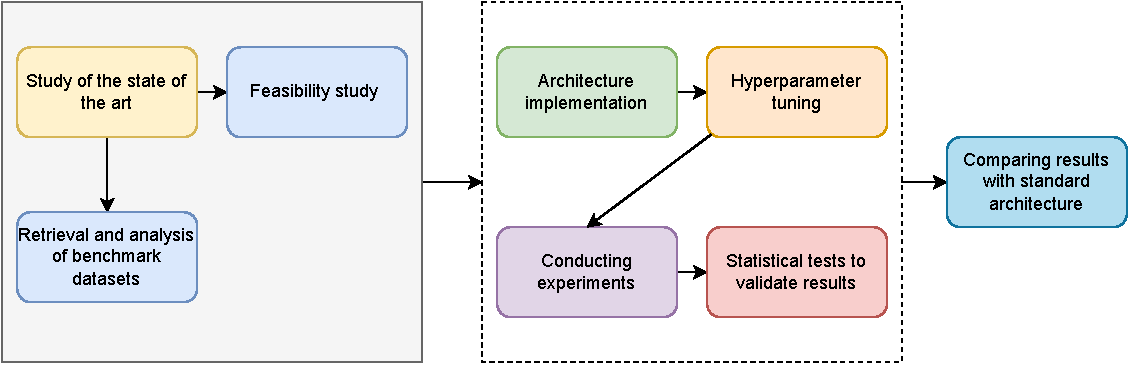
\includegraphics[width=\textwidth,height=4cm]{images/execution plan.pdf}
  \caption{Overview of the experiment pipeline}
  \label{pipeline}
\end{figure*}
CIFAR-10 and CIFAR-100 are benchmark datasets commonly used for image classification tasks in computer vision research. Both datasets were created by the Canadian Institute for Advanced Research (CIFAR).

CIFAR-10 consists of 60,000 32x32 color images in 10 classes, with 6,000 images per class. The 10 classes are: airplane, automobile, bird, cat, deer, dog, frog, horse, ship, and truck.

CIFAR-100, on the other hand, consists of 60,000 32x32 color images in 100 classes, with 600 images per class. The 100 classes are grouped into 20 superclasses, each containing 5 subclasses. For example, the "aquatic mammals" superclass contains the "beaver", "dolphin", "otter", "seal", and "whale" subclasses.

Both datasets are commonly used to train and evaluate machine learning models, particularly in the field of deep learning. Because the images are relatively small and low-resolution, the datasets can be trained on standard hardware without requiring a large amount of memory or computational resources. Additionally, because the images contain a wide variety of objects and backgrounds, they are a good benchmark for evaluating a model's ability to generalize to new, unseen data.

Over the years, many state-of-the-art models have been trained and evaluated on these datasets, including various convolutional neural network (CNN) and Vision Transformer (ViT) architectures. Achieving high accuracy on these datasets has become a standard benchmark for evaluating the performance of image classification models.
